% !TeX program = xelatex
% Main paper. Full established proofs are in the preserved proof supplement.
\documentclass[10pt,a4paper]{article}
\usepackage[margin=25mm,headheight=13pt,headsep=6mm,footskip=10mm]{geometry}
\usepackage{fontspec}
\IfFontExistsTF{Nimbus Roman}{\setmainfont{Nimbus Roman}}{\setmainfont{TeX Gyre Termes}}
\IfFontExistsTF{Nimbus Sans}{\setsansfont{Nimbus Sans}[Scale=MatchLowercase]}{\setsansfont{TeX Gyre Heros}[Scale=MatchLowercase]}
\setmonofont{Latin Modern Mono}[Scale=.85]
\usepackage{amsmath,amssymb,amsthm,mathtools}
\usepackage{unicode-math}
\IfFontExistsTF{Asana Math}{\setmathfont{Asana Math}}{\setmathfont{Latin Modern Math}}
\usepackage{graphicx,booktabs,tabularx,array,caption,microtype,fancyhdr,placeins,needspace}
\usepackage[unicode,hidelinks]{hyperref}
\hypersetup{pdftitle={Correction Delays in Shared-Scale Attention},pdfauthor={},pdfsubject={Archived research report; restricted results and unestablished native transfer}}
\newtheorem{theorem}{Theorem}
\newtheorem{proposition}[theorem]{Proposition}
\newtheorem{corollary}[theorem]{Corollary}
\newtheorem{lemma}[theorem]{Lemma}
\newenvironment{sketch}{\begin{proof}[Proof sketch]}{\end{proof}}
\newcommand{\B}{\mathcal B}
\newcommand{\E}{\mathbb E}
\newcommand{\J}{\mathrm J}
\newcommand{\F}{\mathrm F}
\newcommand{\R}{\mathbb R}
\newcommand{\norm}[1]{\lVert#1\rVert}
\newcolumntype{Y}{>{\raggedright\arraybackslash}X}
\setlength{\parindent}{1em}\setlength{\parskip}{2pt}
\setlength{\jot}{3pt}\setlength{\emergencystretch}{1.5em}
\setlength{\textfloatsep}{10pt}\setlength{\intextsep}{9pt}
\renewcommand{\arraystretch}{1.13}
\captionsetup{font=small,labelfont=bf,justification=justified,singlelinecheck=false,skip=5pt}
\pagestyle{fancy}\fancyhf{}
\fancyhead[L]{\footnotesize Shared-Scale Attention}
\fancyhead[R]{\footnotesize Archive v0.6}
\fancyfoot[C]{\thepage}\renewcommand{\headrulewidth}{.2pt}
\widowpenalty=10000\clubpenalty=10000\raggedbottom
\begin{document}
\begin{center}
{\fontsize{17}{20}\selectfont\bfseries Correction Delays in Shared-Scale Attention}\par
\vspace{4pt}{\small Archived research report --- v0.6-archive --- 8 October 2026}
\end{center}
\vspace{3pt}
\noindent\textbf{Abstract.}
Attention must rank useful information correctly and assign it sufficient weight. In a restricted normalized population model, learning a shared direct scale can exponentially delay correction under squared copy loss, while fixed scale corrects the stated initialization family in polynomial time. Separate exact-real gradient-descent results cover specified finite budgets. Controlled numerical studies show that the outcome changes with loss, scale parameterization, key geometry, query sharing, and trainable information pathways. An attention-only three-head Value/Output model has diverse-mixture readout representations, yet the registered wrong-ranking, low-risk bypass was not learned on its saved grid. A post-hoc fixed-attention analysis finds a large required-versus-actual coefficient gap and a small resolved residual rate; its cumulative attribution remains unresolved. In pretrained Swin and Qwen experiments, a freezing benefit does not replicate across training seeds, a first-layer score reduction does not reduce Confusable decoys, and the tested all-layer radial direction lowers Neutral and Confusable loss together. These results do not establish a general native scale-mediated bottleneck or a practical training prescription. The project ended after STEP18; this report archives its restricted results, negative evidence, and limitations.

\section{Introduction}
Normalized attention separates score ordering from concentration. Query and key directions determine which token ranks first; a positive scale controls how strongly softmax favors the current ordering. Query--key normalization and learned scales are used in language and vision models \cite{henry2020,liu2022}. When the ordering is initially wrong, greater concentration need not accelerate its correction.

We asked when shared-scale learning delays information-selection correction, whether learned readout paths can resolve output errors without correcting attention ranks, and whether related effects are observable in actual pretrained models. The restricted construction fixes opposite keys and a value readout, with one correctly ranked and one misranked group. For direct-scale Copy-MSE, its joint gradient flow obeys
\[
T_0^\J(\rho;\xi)=\exp\!\left((c_\xi+o_{\B}(1))/\sqrt{\rho}\right),
\]
where $\rho$ is a specified direction-to-scale rate ratio and $c_\xi$ is initialization-dependent. Fixed-scale correction and separate exact-real Cartesian GD results retain their stated domains; no native effective $\rho$ is inferred.

The transfer question remained open after the experiments. Swin's full-training error-area contrast changes sign across two seeds. Qwen exhibits controlled distractor errors, but the two tested gain interventions do not support the selective scale explanations. Later controlled studies separate loss tails, scalar coordinates, key geometry, Q sharing, a raw Key--Value path, and attention-only V/O learning. Their conditional outcomes do not convert the native evidence into confirmation.

This is an archived research record. We preserve established restricted mathematics, controlled observations, and unestablished native transfer as distinct evidence levels. No new theorem extension, training experiment, static readout optimization or trajectory integration was performed for this closeout. All existing sources and negative decisions remain unchanged; the public record omits private or rights-uncertain input material.

\section{Related work}
\paragraph{Scale, normalization, and optimization.}
Query--key normalization introduces an explicit learned attention scale \cite{henry2020}; Swin V2 uses scaled cosine attention with a capped log-scale \cite{liu2022}. Agarwala et al.\ study temperature-dependent dynamics for softmax cross-entropy \cite{agarwala}. Tian et al.\ analyze different learning speeds in attention and decoder components \cite{tian2023}. Unequal speeds are not inherently harmful: two-timescale analyses can also establish convergence \cite{marion2023}. Kosson et al.\ study expected angular updates in rotational equilibrium \cite{kosson}. Their rotation estimates are not a conversion from measured Transformer updates to the coefficient $\rho$ in our model.

\paragraph{Selection, concentration, and loss dependence.}
Max-margin analyses describe limiting token selection and convergence under gradient-based optimization \cite{tarzanaghmax,vasudeva}. Zhai et al.\ connect attention entropy collapse with instability \cite{zhai2023}; Prieto et al.\ distinguish numerical softmax collapse and delayed generalization \cite{prieto2025}. Our delay exists in exact-real dynamics and need not involve a numerical zero. Closest to the loss comparison here, Varre et al.\ study a trainable value--softmax model $L(V\sigma(a))$, including logistic and square losses, and prove polarization and ordering properties under specified initialization \cite{varre}. We instead fix the value readout, separate a shared scalar from two directions, and quantify correction of an imposed wrong ranking. Concentration alone does not identify this correction delay.

\paragraph{Conservation and generalization.}
Conservation laws for attention and residual networks are studied by Marcotte et al.\ \cite{marcotte2025}. Our invariant is a tool for the time analysis, not a standalone claim that conservation in attention is new. Length-dependent scaling is studied by Nakanishi \cite{nakanishi}, Veli\v{c}kovi\'c et al.\ \cite{velickovic2025}, and Hilton-Jones et al.\ \cite{hiltonjones}. Their settings and length laws differ from our repeated-key test family. Sagawa et al.\ distinguish fitting a training group from generalizing to it \cite{sagawa2020}; this distinction is central to our Swin tests. Controlled reading-comprehension distractors build on Jia and Liang \cite{jia2017}, rather than constituting a new data-manipulation method.

\section{Model and main results}\label{sec:theory}
\subsection{Directions, scale, and the prediction task}
Choose group $i=1,2$ with probabilities $p_1=1-p$ and $p_2=p$. A normalized query direction $w_i/r_i$ has correct-minus-incorrect score gap
\begin{equation}
d_i=2\sin\phi_i,\qquad w_i=r_i(\cos\phi_i,\sin\phi_i).
\label{eq:gaps}
\end{equation}
An attention embedding uses the two columns in separate planes of $\R^4$, one-hot group queries, and fixed opposite keys in each plane. No group label or correct index is an extra score feature. The planes are invariant, and the gradient is tangent to each column. Thus $r_i$ is constant under gradient flow, but generally grows under gradient descent.

For one correct key and $M\ge1$ repeated incorrect keys, draw independent values $V_0,\ldots,V_M\in\{-1,1\}$ uniformly. The predictor is the attention-weighted sum and the target is $V_0$. At evaluation scale $b\ge0$, averaging over values gives
\begin{equation}
\E[(f-V_0)^2]=\ell_M(bd_i),\qquad
\ell_M(z)=\frac{M(M+1)}{(e^z+M)^2}.
\label{eq:risk}
\end{equation}
The cross terms vanish by independence and zero means. Repeated keys do not mean repeated values.

Training uses $M=1$ and the loss with no factor $1/2$,
\begin{equation}
J=\sum_i p_i\ell(\beta d_i),\quad
\ell(z)=\frac{2}{(1+e^z)^2},\quad
\psi(z)=-\ell'(z)=\frac{4e^z}{(1+e^z)^3}.
\label{eq:copyloss}
\end{equation}
Joint learning updates the direct scalar at rate one and Cartesian query columns at rate $\rho$:
\begin{equation}
\dot\beta=F:=\sum_i p_i d_i\psi(\beta d_i),\qquad
\dot\phi_i=\frac{2\rho p_i\beta\cos\phi_i}{r_i^2}\psi(\beta d_i).
\label{eq:flow}
\end{equation}
The scalar is projected only at zero. Fixed-scale learning, denoted $\F$, keeps the same instance's $\beta_0$ and uses the same direction updates. Define $T_0^A=\inf\{t:d_2^A(t)\ge0\}$ for either policy $A$. Positive-margin attainment is a different event: $T_\gamma^\F=\inf\{t:\min_i d_i^\F(t)\ge\gamma\}$.

\subsection{Uniform sharp delay}
Let $\xi=(p,\beta_0,r_1,r_2,g_0,\vartheta)$ and
\begin{equation}
\begin{split}
\B={}&[.049,.051]\times[.99,1.01]\times[.95,1.05]^2\\[-2pt]
&\times[.19,.21]\times[.79,.81].
\end{split}\label{eq:box}
\end{equation}
Set $\phi_{1,0}=\arcsin(g_0/2)$, $\phi_{2,0}=-\vartheta$, and $a_0=2\sin\vartheta$. Initial conditions do not depend on $\rho$. Throughout $\B$, $0<g_0<a_0/2$, so group 2 starts with gap $-a_0$. The reference point is $\xi_0=(.05,1,1,1,.2,.8)$. Decimal endpoints are exact rationals.

\begin{theorem}[Sharp gradient-flow correction]\label{thm:sharp}
For \eqref{eq:flow} on \eqref{eq:box}, solutions exist at every finite time and $\beta\ge.01$. Let $B_\rho=\sup_{t\le T_0^\J}\beta(t)$ and
\begin{equation}
b_\xi=r_1\sqrt{\log\frac{1-g_0^2/4}{1-a_0^2/16}},\qquad c_\xi=a_0b_\xi.
\label{eq:coeff}
\end{equation}
There is a common positive cutoff below which $T_0^\J<\infty$. For every $\epsilon>0$ there is $\rho_\epsilon>0$ such that, for all $\xi\in\B$ and $0<\rho<\rho_\epsilon$,
\begin{equation}
\left|\sqrt\rho\log(1+T_0^\J)-c_\xi\right|<\epsilon,
\qquad \left|\sqrt\rho B_\rho-b_\xi\right|<\epsilon.
\label{eq:sharp}
\end{equation}
\end{theorem}
\begin{sketch}
The exact conserved quantity is
\begin{equation}
Q=\rho\beta^2/2+\sum_i r_i^2\log\cos\phi_i.
\label{eq:inv}
\end{equation}
Before correction, $a=-d_2$ decreases. With $u=\sqrt\rho\beta$, conservation gives the limiting easy-gap curve
$G_\xi(u)=2\sqrt{1-(1-g_0^2/4)e^{-u^2/r_1^2}}$, with $G_\xi(b_\xi)=a_0/2$. The finite-$\rho$ formula retains $\rho\beta_0^2$ and the second angle's motion.

At frozen initial angles, the opposing/positive scale-force ratio is bounded by
\[
\frac{pa_0}{(1-p)g_0}e^{-(a_0-2g_0)\beta}(1+e^{-g_0\beta})^3<.94.
\]
Each beta-dependent factor in this upper bound decreases. A separate finite-scale argument then establishes live entry; frozen positivity is not a trajectory assumption. Fix a buffer $\lambda>0$ before choosing $\rho$. Up to the first hit of $u=(1-\lambda)b_\xi$, the initially wrong angle moves by $O(\rho)$, uniformly over $\B$. The actual clock is bounded above and below by constant multiples of
\[
\rho^{-1/2}\int \exp\{2uG_\xi(u)/\sqrt\rho+O(\sqrt\rho)\}\,du.
\]
An endpoint bound gives the time lower coefficient; the first hit gives the peak lower coefficient. For the upper bound, fix $v_\xi>b_\xi$. Above it, $2d_1-a$ has a positive margin and
\[
\frac{(\dot u)_+}{-\dot a}\le C_{\B,v}\exp(-\kappa_v b_{\min}/\sqrt\rho).
\]
All positive excursions consume the same total decrease of $a$, at most $a_0$. This bounds the entire peak, without dividing by a vanishing scale velocity. The peak bound and positive scale floor then give a positive lower bound on the correction speed, proving finite correction and the matching time upper bound. Buffers are fixed first, then $\rho$ is made small. Complete uniform estimates are in the proof supplement.
\end{sketch}
At $\xi_0$, $b_\xi=0.3572969934$ and $c_\xi=0.5126183490$. Writing $\rho_1=\rho/r_1^2$ makes the radius dependence of the leading time exponent explicit. It does not remove radius dependence from every finite-time term. The theorem gives a logarithmic coefficient, not a timing prefactor or a useful numerical cutoff for every observed trajectory.

\subsection{An error floor throughout the delayed interval}
Fixed scale reaches both gaps at least $\gamma=1/5$ by $40/\rho$ and keeps them there. For example, a uniform bound for group 2 is $\rho T_{\gamma,2}^{\F}<113875/2992<40$; the extra group-1 time, when needed, is also below this budget.
\begin{corollary}[Persistent population error]\label{cor:floor}
For a common sufficiently small $\rho$, all $\xi\in\B$, all integers $M\ge1$, and every $40/\rho\le t<T_0^\J$,
\begin{equation}
\begin{split}
\inf_{b\ge0}R_M^\J(t;b,\xi)&\ge\frac{pM}{M+1},\\
R_M^\F(t;b_M,\xi)&\le p_{\min}/4,\\
\inf_{b\ge0}R_M^\J(t;b,\xi)-R_M^\F(t;b_M,\xi)&\ge49/4000,
\end{split}\label{eq:floor}
\end{equation}
where $p_{\min}=.049$ and $b_M=\log(4M(M+1)/p_{\min})/(2\gamma)$.
The duration $T_0^\J-40/\rho$ has the same leading logarithmic exponent as $T_0^\J$.
\end{corollary}
\begin{sketch}
For $t<T_0^\J$, $d_2^\J<0$ and $e^{bd_2^\J}\le1$, giving the first bound from \eqref{eq:risk}. Fixed-scale margin persistence gives $\ell_M(b_Md_i^\F)\le p_{\min}/4$. Since $p\ge p_{\min}$ and $M/(M+1)\ge1/2$, subtraction proves the contrast. The uniform positive lower exponent implies $(40/\rho)/T_0^\J\to0$ uniformly, so subtracting that polynomial time does not change the leading exponent.
\end{sketch}
This is a consequence of the direction theorem, not an independent generalization theory. Test values are fresh, but queries and the repeated-key structure remain fixed. The evaluation rule depends on $M$; raw Fixed risk need not be lower. The error difference is MSE, not classification percentage points.

\subsection{Actual gradient descent at a finite budget}
Set $\alpha=\rho\eta$ and evaluate all derivatives at the same pre-update state:
\begin{equation}
w_{i,k+1}=w_{i,k}-\alpha\nabla_{w_i}J_k,\quad
\beta_{k+1}=\max(0,\beta_k-\eta\partial_\beta J_k),\quad
N=\left\lceil\frac{40}{\rho\eta}\right\rceil.
\label{eq:gd}
\end{equation}
No momentum, decay, clipping, radius reset, or extra scale floor is used. If $x_i=2\alpha p_i\beta\cos\phi_i\psi(\beta d_i)/r_i^2$, the exact Cartesian step satisfies
\begin{equation}
\phi_{i,+}=\phi_i+\arctan x_i,\qquad
r_{i,+}^2=r_i^2(1+x_i^2).
\label{eq:polar}
\end{equation}
\begin{theorem}[Two finite-budget GD guarantees]\label{thm:gd}
For every $\xi\in\B$, Joint has $d_{2,k}<0$ for all $0\le k\le N$, and Fixed has both gaps at least $1/5$ by $N$, in either of the following settings:
\[
0<\rho\le10^{-9},\ 0<\eta\le1/5;
\qquad\text{or}\qquad (\rho,\eta)=(10^{-4},1/5).
\]
At the latter setting, $N=2{,}000{,}000$ and $d_{2,k}<-1.38$ throughout. The risk contrast in \eqref{eq:floor} holds at $N$ for all $M\ge1$.
\end{theorem}
\begin{sketch}
For the small-rate interval, a scale-force ratio below one and a discrete exponential bound control $\beta_n$ by $c^{-1}[5+\log(1/\rho)]$. Summing $\beta_k\Delta\beta_k$ bounds both angle movements, including a hypothetical first exiting step. The upper endpoint $10^{-9}$ leaves a strict margin.
At the fixed setting, stop on the first exit from $d_1\le.6$, $\phi_2-\phi_{2,0}\le.02$, $\beta\le20$. Separate force-ratio bounds below and above $\beta=3$, the exact log-cos increment, and actual radius growth exclude both angle exits. If $\beta$ reaches 18, prior easy progress implies $d_1>3/8$, and the remaining force gives $\beta<19.059613<20$. All first exits are excluded. For Fixed, descent bounds total squared-radius growth by $2\alpha J_0$; integer hitting estimates include the final overshoot. The complete proof retains $N\eta$, not $40/\rho$ substituted for a rounded budget.
\end{sketch}
The second guarantee covers the full closed box, not just observed points. It does not fill the interval between $10^{-9}$ and $10^{-4}$ or cover other step sizes at the fixed setting. Neither result is a sharp exponential-time GD theorem.

\section{Loss, coordinates, and controlled information paths}\label{sec:controlled}
\subsection{Existing numerical evidence and the limits of the sharp law}
The prescribed uniform-law records have nine initializations at three rates. At the smallest rate, recorded relative errors of the time coefficient are $1.158$--$1.412\%$ and of the peak coefficient $0.523$--$0.638\%$ (Figure~\ref{fig:uniform}). Coefficients come from initialization, not a fitted curve. At the reference point, $\log(1+T_0)=239.4712589$ versus $c_{\xi_0}/\sqrt{\rho}=236.4532124$; the unnormalized timing prefactor is not established.

All 36 prescribed Cartesian GD paths reached their registered finite budget. Stored Joint end gaps span $[-1.44843,-1.41839]$, and Fixed minimum gaps span $[1.10065,1.26100]$. All 72 common-scale risk contrasts at four test lengths exceed $49/4000$, while 54 raw-scale contrasts favor Joint. These numerical records support the particular comparisons; the theorem's full-box quantifiers follow from the preserved proofs, not from finite samples.

A separate free-QK bridge learned both matrices with finite queries. Fixed first reached $99\%$ correct ranking at 8,250 updates; Joint at 10,000 and 9,750 in two prescribed runs. Joint nevertheless had lower final raw risk. Its matrix rates are not identified with the theorem's $\rho$.

\begin{figure}[!htbp]\centering
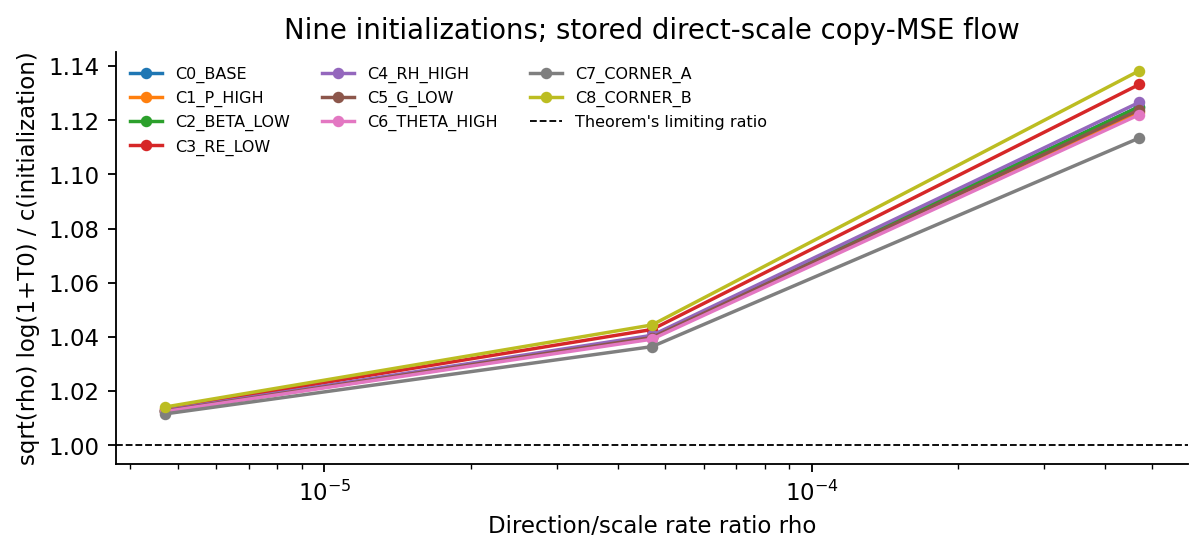
\includegraphics[width=.86\linewidth]{figures/01_restricted_delay.png}
\caption{Stored nine-initialization direct-scale Copy-MSE diagnostics. The normalized log time approaches the initialization coefficient at the tested small rates. Connecting finite observations is not a new uniform proof or time-prefactor estimate.}\label{fig:uniform}
\end{figure}

\subsection{Loss tails and scalar mobility}
A value readout has $\partial_{z_j}L=A_j\langle V_j-f,\nabla_f L\rangle$.
Bounded values and outer gradients give an upper bound but not a matching lower tail: the inner product can cancel. For Copy-MSE, the kernel tails are $4e^{-2z}$ and $4e^{-x}$; for the defined logistic value loss they are $\sigma(-1)e^{-z}$ and $\sigma(1)e^{-x}$. Pointer-CE instead has tails $e^{-z}$ and $1$, so its incorrectly ranked signal does not vanish in this comparison. These are different loss pathways.

If $\dot\beta=m(\beta)F$, the existing local conservation identity is
\[
Q_m=\rho\int_{\beta_0}^{\beta}\frac{u}{m(u)}\,du+
\sum_i r_i^2\log\cos\phi_i.
\]
Direct scale has $m=1$, and Euclidean log-scale flow has $m=\beta^2$.
The original derivation and conditional positive-floor/bounded-cap estimate are preserved in the scope supplement. A general sharp tail law, arbitrary compact initialization region, log-scale double-exponential theorem, Adam transfer and sharp GD escape law were \emph{not established in this project}.

The completed STEP16R comparison fixes three losses, two scalar coordinates and nine rates: 54 joint cells, with matched fixed-scale events. Forty-two corrected; twelve are right-censored at the physical log-clock horizon 300. Censors are lower-bound observations, not stopped optimization or infinite time. Direct Copy-MSE Joint/Fixed time ratios at $\rho=.1,.03,.01,.003,.001$ are $.75443,1.01000,2.40164,40.40868,12709.42$. The sign changes within the tested range (Figure~\ref{fig:loss}); no general phase boundary is fitted.

\begin{figure}[!htbp]\centering
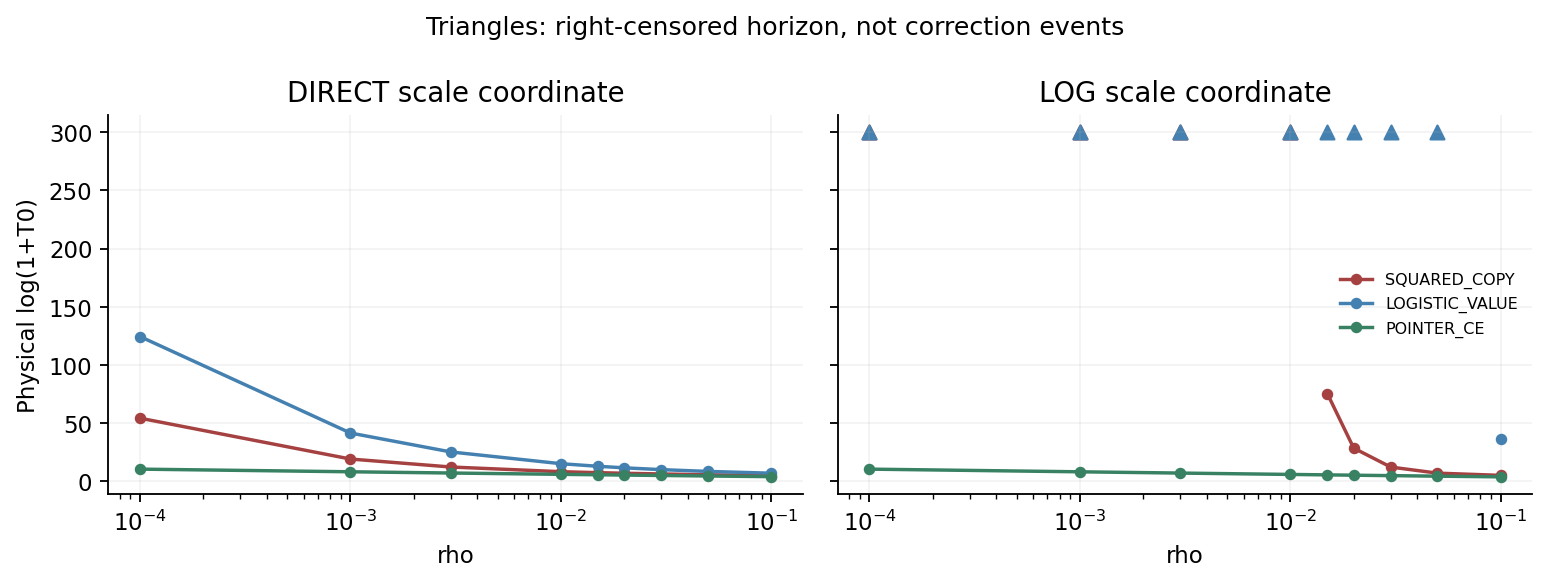
\includegraphics[width=\linewidth]{figures/02_loss_and_scale_coordinate.png}
\caption{The completed fixed loss/coordinate comparison. Triangles indicate right-censored physical log-clock horizons, not attained correction times. Initial conditions and events are shared within the matched comparisons; scalar coordinates are different update policies.}\label{fig:loss}
\end{figure}

\subsection{Key geometry, shared queries, and a distinct raw-value path}
The controlled bridge uses $x_1=(1,0)^T$, $x_2=(1/2,\sqrt3/2)^T$, probabilities $19/20,1/20$, opposite fixed keys and independent sign Values. Four Value combinations and both candidate orders give 16 population rows per law; the STRONG/WEAK raw-input union has 24 rows. This is an exact population average, not a sampled dataset.

STEP16R compares key geometry, shared versus separate Q matrices, and absence/presence of a learned bilinear path $x^TB\sum_jk_jV_j$. Its 32 logical paths reuse eight Fixed slow-time paths across two rates. In STRONG without this path at $\rho=.003$, Joint's wrong-rank occupation is one for shared and separate Q; Fixed improves from $.40625$ to $.12125$ when Q is shared. Thus the larger Joint--Fixed contrast includes improved Fixed correction. Other geometry/rate settings favor Joint. The raw Key--Value path can achieve low output risk while ranking stays wrong, but it reads information unavailable to ordinary attention-only V/O. It is not evidence that every Transformer has the same bypass.

\subsection{Attention-only V/O: representation and finite-horizon learning}
STEP17 removes the raw path. All heads share one $2\times2$ Q matrix and beta, with relative scales $(1/4,1,4)$ for the three-head model. Scalar Value projections $v_h$ are attention-averaged before linear Output mixing $o_h$. The one-head fixed/readout-trained and three-head trained models start with the same effective prediction. Actual $v,o$ are integrated, not direct $c$-GD for $c=v\odot o$.

For one head, $L=(cA-1)^2+c^2(1-A)^2$, with the existing static bound
\[
\min_cL=\frac{(1-A)^2}{A^2+(1-A)^2}\ge\tfrac12\quad(A\le\tfrac12).
\]
Replicated identical mixtures retain this bound. With three diverse mixtures, a shared signed exact readout can exist if $[{\bf1};A_1;A_2]$ is invertible; that is representation, not learning attainment.

The study has 24 logical paths: six parent integrations reused and twelve new Main integrations, with Fixed paths mapped to both rates. The common horizon is slow time $\tau=40$, with 401 nodes per path. The registered primary on STRONG/H3/Joint/$\rho=.003$ is the trapezoid occupation of all-head misranking with both group MSEs at most $.1$. It is $P17=0$, including numerical ambiguity range $[0,0]$. All logical auxiliary occupations are also zero. The other five unique H3 paths meet the loss targets after observed rank correction; Figure~\ref{fig:vo} retains all six. No continuous-time absence theorem or generic multi-head impossibility follows.

\begin{figure}[!htbp]\centering
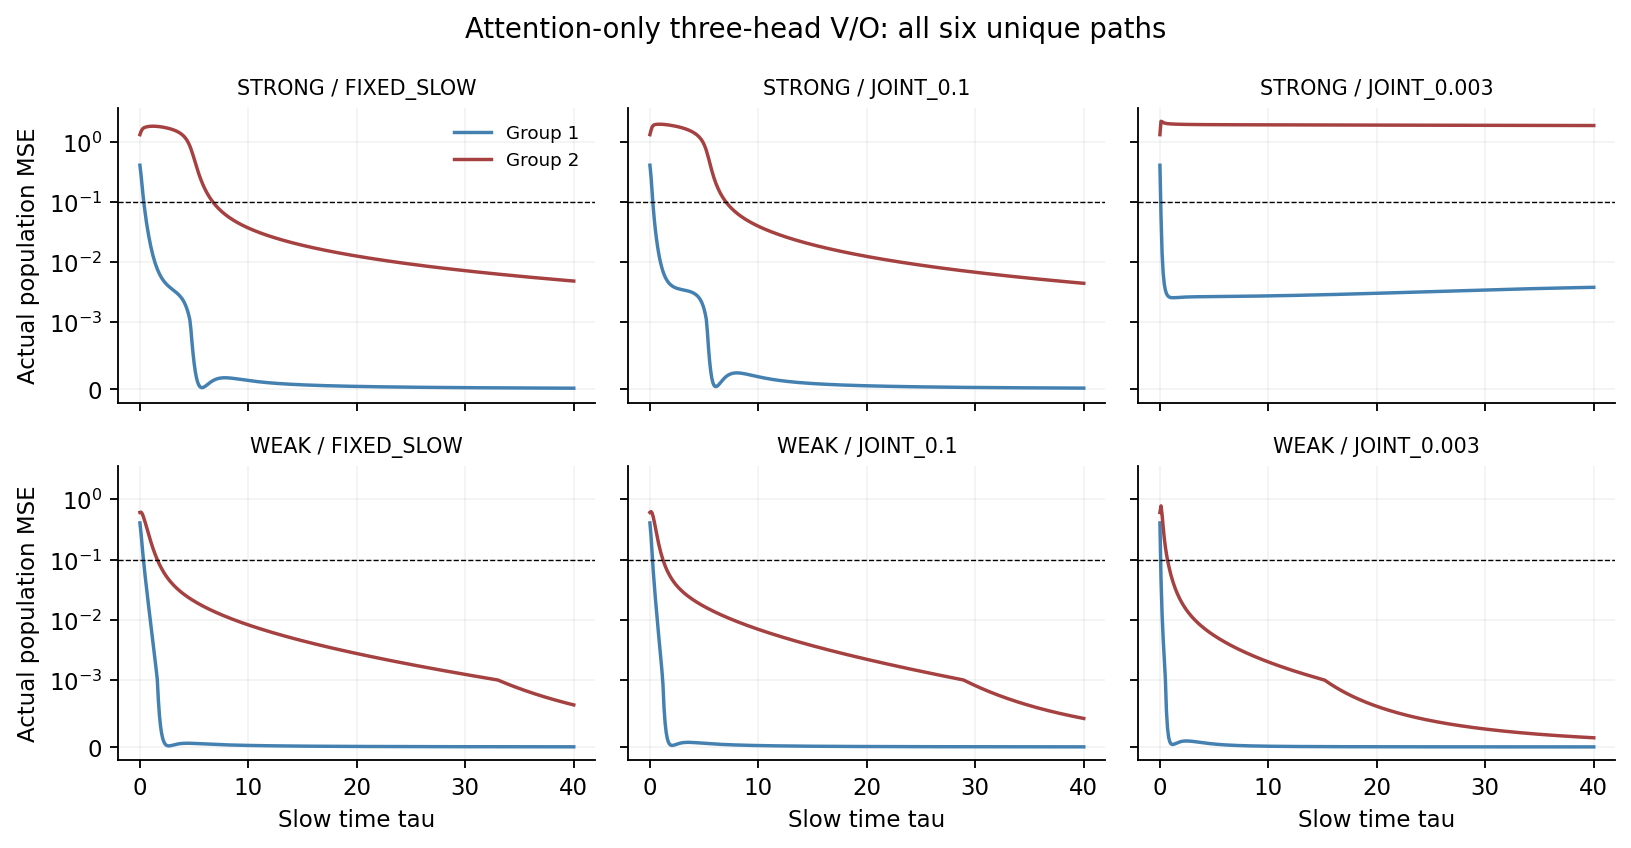
\includegraphics[width=\linewidth]{figures/05_attention_vo_actual_losses.png}
\caption{Actual population MSE for all six unique H3 paths. The horizontal threshold is $.1$ per group. Fixed curves are one slow-time trajectory per geometry, not separate independent runs for each rate.}\label{fig:vo}
\end{figure}

\subsection{Saved-state readout requirements and local dynamics}
STEP18 analyzes those six existing paths at 401 nodes without new integration.
With $M_i=[A_i^T;(1-A_i)^T]$, $r_i=M_ic-(1,0)^T$ and
$D=[\sqrt{p_1}M_1;\sqrt{p_2}M_2]$, it separates actual coefficients, weighted LS representation, and minimum norm for \emph{each} $L_i\le.1$.
At STRONG/H3/Joint/$\rho=.003$, $\tau=40$,
\[
L_1=.0038081163,\quad L_2=1.8474173534,\quad
\|c_{\rm actual}\|_2=.9921652.
\]
The recorded numerical target-norm bracket is
$[2964.683830041,2964.683840466]$, about $2988.09$ times actual.
The weighted zero-residual LS coefficient norm is instead about $4342.68$.
A valid analytical norm-ball loss lower bound exceeds $.1$ at the current norm.
These are fixed-attention comparisons; no oracle is injected into the learning path.

In slow time the factorized dynamics satisfy
\[
\begin{aligned}
g_c&=2D^Tr,\qquad G=\operatorname{diag}(v_h^2+o_h^2),\\
\dot c&=-Gg_c,\qquad \dot r=-2DGD^Tr+\dot D c.
\end{aligned}
\]
$G$ remains nonzero. At the primary endpoint, $D\sqrt G$ has smallest resolved singular value about $1.44629\times10^{-4}$, and $99.997769\%$ of the current residual energy lies in its smallest resolved subspace. This is instantaneous geometry, not a percentage causal attribution of failed learning or a future convergence time.

For the same weighted objective, $\dot J_{VO}=-g_c^TGg_c\le0$,
$\dot J_Q=-\|\nabla_WJ\|_F^2\le0$, and projected scale contributes nonpositively. Moving attention does not raise weighted $J$ to cancel V/O improvement under this flow, although individual group terms can be positive. The required coefficient norm and conditioning can worsen while weighted $J$ falls.

All 18 stored $.1$- versus $.2$-grid cumulative derivative comparisons remain
\texttt{INTEGRAL\_UNRESOLVED}. Local identities do not license cumulative causal fractions. Figure~\ref{fig:readout} presents the static requirement separately from actual coefficients; no new optimization was performed for the archive.

\begin{figure}[!htbp]\centering
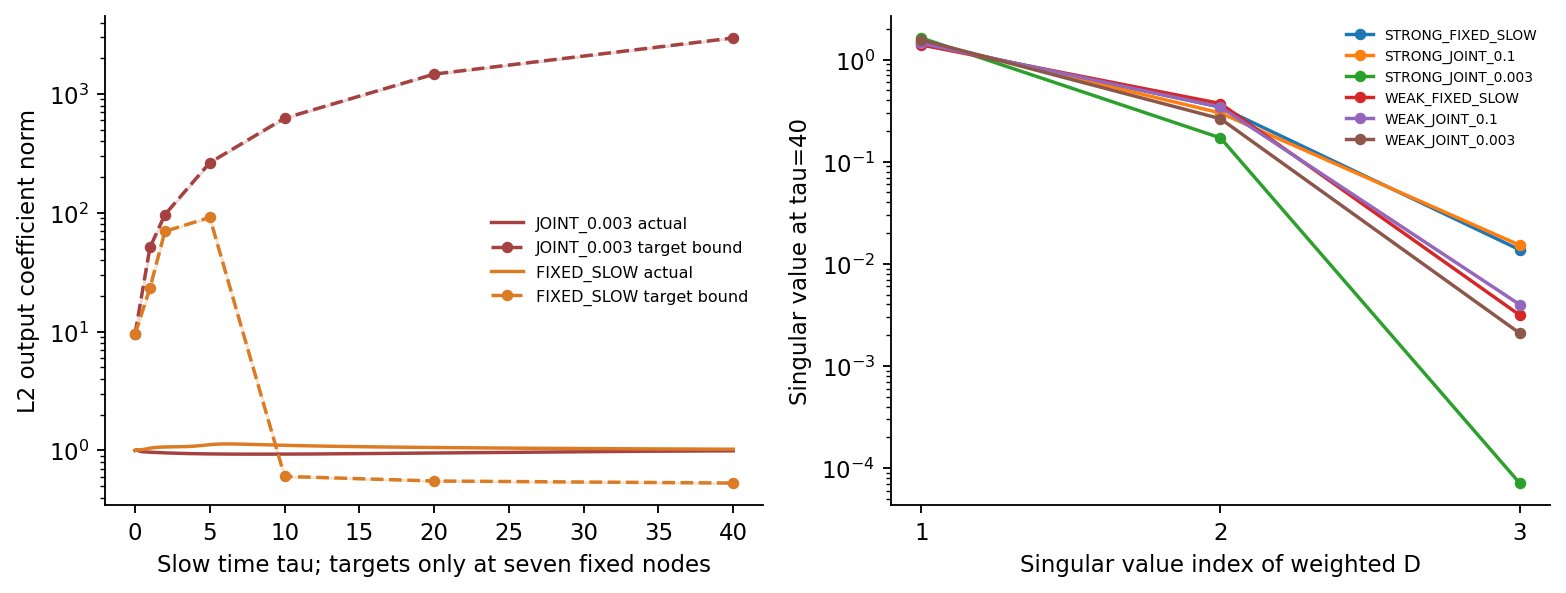
\includegraphics[width=\linewidth]{figures/06_readout_required_norm_and_spectrum.png}
\caption{Left: actual output norms and previously computed target-norm intervals at seven fixed states on the primary and Fixed paths. Right: weighted-$D$ endpoint spectra for all six unique H3 paths. Static readout requirements are not learned performance or a GF time bound.}\label{fig:readout}
\end{figure}
\FloatBarrier
\section{Tests in pretrained Transformers}\label{sec:pretrained}
\subsection{Swin: distinct metrics and a training benefit that does not replicate}
The preceding six-run pilot used a different clipping control and a validation-CE primary. Its Native-minus-Hold integrated Hard CE contrasts were $+.058145$ and $+.469775$, while final WGA was higher for Native in both seeds ($.759398$ versus $.503759$; $.691729$ versus $.661654$). Temporal effects, opposing hard-group changes, and incorrect-answer confidence reconcile those quantities; they do not identify a consistent training optimization delay. The later full-training census and common clipping address a different comparison, without replacing that pilot's primary.

We fine-tune ImageNet-pretrained Swin V2 Tiny on Waterbirds, predicting bird type from images with correlated backgrounds. The two background-conflicting groups contain 184 and 56 training images. These are data groups, not certified negative attention gaps. AdamW uses backbone/scale LR $5\times10^{-5}$, head LR $5\times10^{-4}$, matrix weight decay $.05$, zero decay for bias/norm/scale, a 100-step warmup, and 1,000 updates at effective batch 64.

In the controlled pair, both policies compute scale gradients and include them in the same global clipping norm (threshold one); only one policy omits scale from the optimizer. The primary is clean, group-macro classification error on all 240 conflicting training images, integrated over the registered 100-step grid. Figure~\ref{fig:swin} and Table~\ref{tab:swin} show the sign reversal. Worst-group validation accuracy favors fixed scale in both seeds, while frequency-weighted overall validation accuracy favors learned scale. Neither secondary replaces the failed training-primary replication.
\par
\begin{table}[!htbp]\centering\small
\caption{Controlled Swin runs. $U$ is integrated mean training error. The contrast is learned minus fixed scale. Validation columns give learned/fixed percentages.}\label{tab:swin}
\begin{tabular*}{\linewidth}{@{\extracolsep{\fill}}lrrrrr@{}}\toprule
Seed & $U_\J$ & $U_\F$ & Contrast (pp) & WGA (\%) & Overall (\%)\\\midrule
1103 & .061296584 & .059860248 & $+.143634$ & 72.18/75.94 & 92.16/91.33\\
1104 & .064518634 & .066440217 & $-.192158$ & 65.41/69.92 & 89.91/86.57\\\bottomrule
\end{tabular*}
\end{table}
\par
Swin uses $\beta=\exp(\min(s,\log100))$ with a positional bias outside the scale. The model, loss, optimizer, and learned readout differ from the theorem. The maximum recorded relative scale increase in seed 1103 was about $.653\%$, with mixed signs across coordinates. Net scale change and noisy weight rotation do not determine an effective $\rho$; we do not classify these runs as a theoretically certified benign regime.


\begin{figure}[!htbp]\centering
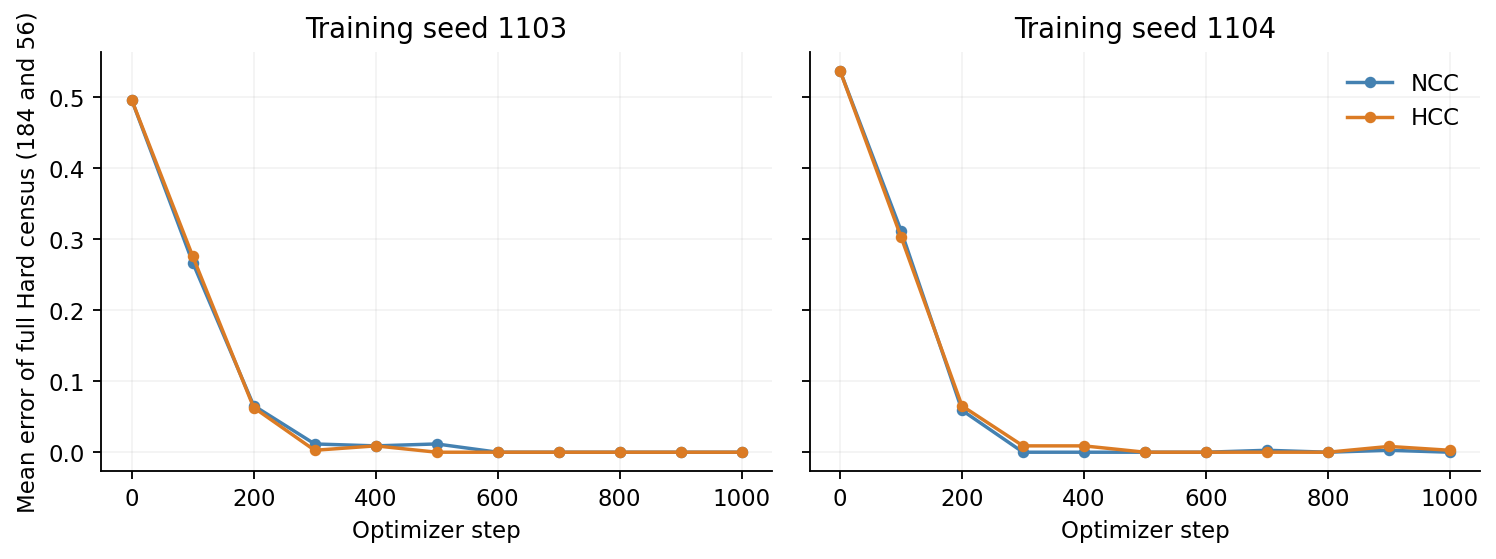
\includegraphics[width=\linewidth]{figures/03_swin_seed_reversal.png}
\caption{Clean Training Hard error on the complete 240-image census, with equal weight for the 184-image and 56-image groups. Seeds remain separate; the small integrated policy contrasts have opposite signs. This is not elapsed-time acceleration.}\label{fig:swin}
\end{figure}
\subsection{Qwen: directed distractor errors, but no selective scale effect}
We use a fixed Qwen3-0.6B checkpoint~\cite{qwen} with 164 SQuAD-derived and 92 QED-derived questions~\cite{rajpurkar2016,qed2021}, one per document cluster. Each question has evidence only (EO), evidence plus a Neutral distractor (N), a Confusable distractor (C), question only, and evidence with the answer replaced (CF). N and C share the question, evidence, decoy answer, token count, and location; only the distractor entity changes. In the original 128-question held-out partition, designated-decoy outputs increase from $10$ to $22$, or $9.375$ percentage points. EO and CF accuracies are $108/128$ and $107/128$. This establishes a controlled input effect, not a scale mechanism.

A frozen first-layer Q/K gain intervention multiplies both gains by $\sqrt r$ for $r=.8,1,1.25$. At a fixed prefix this changes pre-mask scores by $r$ while preserving local Q/K directions. On the reused held-out partition, the N/C decoy counts are $9/22$, $10/22$, and $11/23$. The registered reduction contrast is $-1/128$: reducing the first-layer score does not reduce C decoys. Downstream representations can still change; this is not a direction-correction experiment.

The dataset is synthetic in part. All paired distractor entities contain ``Vale'' and 197 Neutral names start with ``London''. The designated name Alex Voss recurs in 32 cases. The cohort changed from the original SQuAD-only proposal, and historical static-trial compliance remains false. Strict exact match also distinguishes a short answer from an explanatory sentence containing it. All inputs and scoring rules remain fixed, but these facts limit the task's scope. The partitions are not certified absent from pretraining. In the later interventions they are explicitly reused, not fresh confirmation data.

\subsection{An all-layer test of local scale-gradient conflict}\label{sec:p15}
At the same Qwen checkpoint, let $\theta_l$ concatenate the query/key RMSNorm gains of layer $l$. Define the Euclidean common-radial projection
\begin{equation}
P_lg_l=\theta_l\frac{\langle\theta_l,g_l\rangle}{\norm{\theta_l}^2},\quad
G_{DN}=\frac1{128}\sum_{i\in\mathrm{DEV},N}\nabla_\theta L_i,\quad
v=-PG_{DN}/a_{\max},
\label{eq:proj}
\end{equation}
where $a_{\max}=\max_l|\langle\theta_l,G_{DN,l}\rangle|/\norm{\theta_l}^2$ normalizes the largest layer-wise relative gain change to one. The direction is selected using DEV Neutral correct-answer loss alone and locked before other gradients are aggregated. Each layer's Q/K gains move by the same relative factor, but different layers can move in opposite directions. Residual gain gradients outside this projection are not pure QK direction gradients.

The loss is mean correct-answer-token CE, with EOS differentiated separately. All 56 gain tensors (7,168 coordinates) are differentiated; other weights remain frozen without detaching paths to the gains. For reused held-out condition $X$, let $B_X=\langle G_X,v\rangle$. The proposed conflict predicts $B_N<0$ but $B_C>0$. Instead,
\begin{equation}
B_N=-2.469364,\quad B_C=-2.978170,\quad
B_{EO}=-1.607058,\quad B_{CF}=-1.133221.
\label{eq:p15}
\end{equation}
The answer loss decreases in all four conditions. The negative DEV-N derivative is true by construction; the held-out values are measurements. Table~\ref{tab:p15} and Figure~\ref{fig:p15} confirm the signs by independently applying four small displacements from the original gains, not by accumulating updates.
\par
\begin{table}[!htbp]\centering\small
\caption{Reused held-out Qwen inputs, $n=128$ per condition. Slopes are nat/answer-token per unit $t$; changes are nat/answer-token. $t=.005$ permits a maximum $.5\%$ gain displacement.}\label{tab:p15}
\begin{tabular*}{\linewidth}{@{\extracolsep{\fill}}lrrrr@{}}\toprule
Condition & Base CE & $B_X$ & $\Delta L(+.0025)$ & $\Delta L(+.005)$\\\midrule
EO & .647118 & $-1.607058$ & $-.00397324$ & $-.00785683$\\
N  & 1.139906 & $-2.469364$ & $-.00612428$ & $-.01214950$\\
C  & 1.278239 & $-2.978170$ & $-.00738558$ & $-.01465411$\\
CF & .501644 & $-1.133221$ & $-.00280028$ & $-.00553571$\\\bottomrule
\end{tabular*}
\end{table}
\par
\par
\begin{figure}[!htbp]\centering
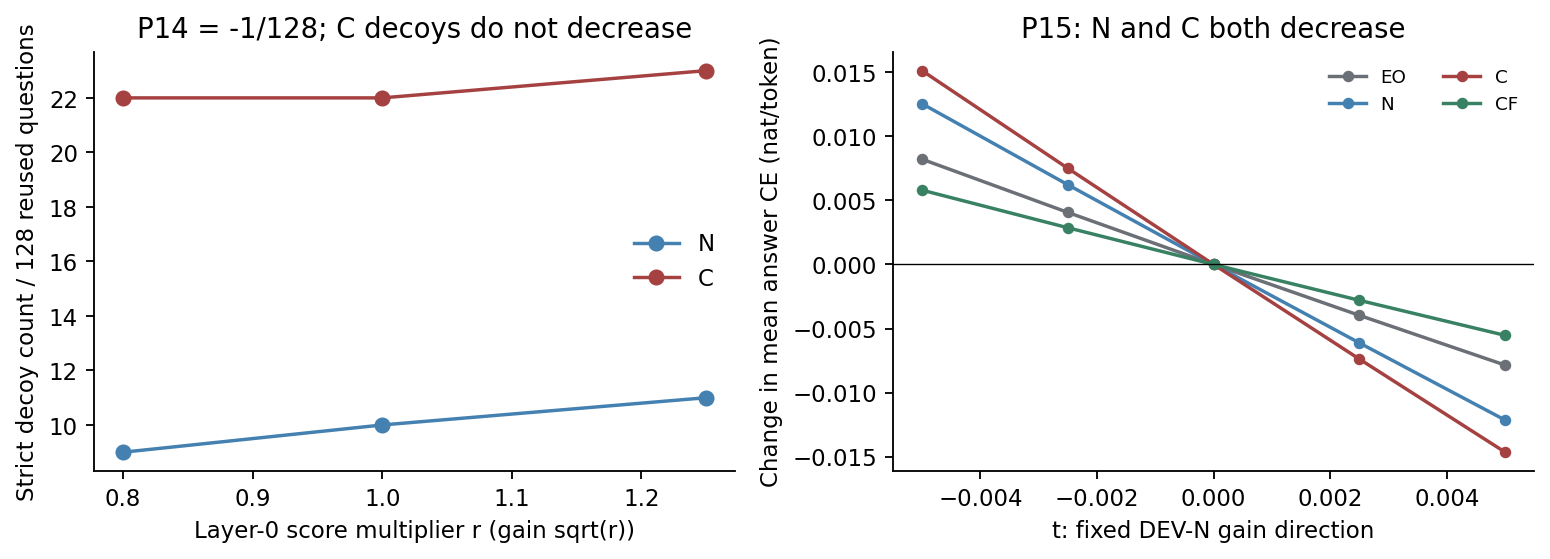
\includegraphics[width=\linewidth]{figures/04_qwen_opposed_and_joint_decrease.png}
\caption{Left: the first-layer intervention does not reduce Confusable designated decoys. Right: one DEV-Neutral-derived gain direction lowers each condition's mean answer CE. The second test uses no optimizer step or free generation.}\label{fig:p15}
\end{figure}
\par
Among the 128 C inputs, 111 directional derivatives are negative and 17 positive; eight layer contributions are positive and twenty negative. These parts are disclosed, not used to choose another primary. Central differences agree with the registered slopes at the tested resolution. The experiment therefore does not support the selected initial scale-conflict explanation. It does not prove that conflict is absent in every direction, parameterization, or future training state. The directions concern Euclidean gains, not AdamW updates, and no generated-answer improvement is measured.
\FloatBarrier

\section{Scope, limitations, and closure}\label{sec:discussion}
The established mathematics retains fixed opposite keys, prescribed initial misranking, population gradients and a fixed readout. Its fresh-value risk is not generalization to arbitrary queries. Loss tails, scalar coordinates, geometry and learned information paths affect the controlled results; no one comparison supplies a universal optimization rule.

Within the stated restricted task, fixed-scale correction followed by the length-dependent evaluation rule provides a constructive alternative. That conditional construction is not a demonstrated native-model speed, memory, accuracy or hallucination improvement. Swin/Qwen use different parameterizations, multilayer representations, losses and optimizers, and their negative or mixed results are not reclassified as a theoretically certified benign regime.

The record therefore distinguishes \emph{proved restricted results}, \emph{observed controlled behavior}, and \emph{native effects not established}. It neither rejects every possible scale mechanism nor recommends freezing scales generally. The project ended after STEP18. Its theorem scope, conditional numerical results, adverse native evidence, unresolved cumulative attribution and redistribution exclusions are preserved; no further sweep or experiment is scheduled.
\begin{thebibliography}{99}
\setlength{\itemsep}{3pt}
\bibitem{henry2020} Alex Henry, Prudhvi Raj Dachapally, Shubham Shantaram Pawar, and Yuxuan Chen. Query-Key Normalization for Transformers. \emph{Findings of EMNLP}, 2020. \href{https://aclanthology.org/2020.findings-emnlp.379/}{ACL Anthology}.
\bibitem{liu2022} Ze Liu et al. Swin Transformer V2: Scaling Up Capacity and Resolution. \emph{CVPR}, 2022. \href{https://arxiv.org/abs/2111.09883}{arXiv:2111.09883}.
\bibitem{agarwala} Atish Agarwala, Jeffrey Pennington, Yann Dauphin, and Sam Schoenholz. Temperature check: theory and practice for training models with softmax-cross-entropy losses. Preprint, 2020, \href{https://arxiv.org/abs/2010.07344}{arXiv:2010.07344}.
\bibitem{tian2023} Yuandong Tian, Yiping Wang, Beidi Chen, and Simon Du. Scan and Snap: Understanding Training Dynamics and Token Composition in 1-layer Transformer. \emph{NeurIPS}, 2023. \href{https://arxiv.org/abs/2305.16380}{arXiv:2305.16380}.
\bibitem{marion2023} Pierre Marion and Rapha\"el Berthier. Leveraging the two timescale regime to demonstrate convergence of neural networks. \emph{NeurIPS}, 2023. \href{https://arxiv.org/abs/2304.09576}{arXiv:2304.09576}.
\bibitem{kosson} Atli Kosson, Bettina Messmer, and Martin Jaggi. Rotational Equilibrium: How Weight Decay Balances Learning Across Neural Networks. \emph{ICML}, PMLR 235:25333--25369, 2024. \href{https://proceedings.mlr.press/v235/kosson24a.html}{PMLR}.
\bibitem{tarzanaghmax} Davoud Ataee Tarzanagh, Yingcong Li, Xuechen Zhang, and Samet Oymak. Max-Margin Token Selection in Attention Mechanism. \emph{NeurIPS}, 2023. \href{https://proceedings.neurips.cc/paper_files/paper/2023/hash/970f59b22f4c72aec75174aae63c7459-Abstract-Conference.html}{Proceedings}.
\bibitem{vasudeva} Bhavya Vasudeva, Puneesh Deora, and Christos Thrampoulidis. Implicit Bias and Fast Convergence Rates for Self-attention. \emph{TMLR}, 2025. \href{https://arxiv.org/abs/2402.05738}{arXiv:2402.05738}.
\bibitem{zhai2023} Shuangfei Zhai et al. Stabilizing Transformer Training by Preventing Attention Entropy Collapse. \emph{ICML}, PMLR 202:40770--40803, 2023. \href{https://proceedings.mlr.press/v202/zhai23a.html}{PMLR}.
\bibitem{prieto2025} Lucas Prieto, Melih Barsbey, Pedro A. M. Mediano, and Tolga Birdal. Grokking at the Edge of Numerical Stability. \emph{ICLR}, 2025. \href{https://iclr.cc/virtual/2025/poster/29501}{Conference record}.
\bibitem{varre} Aditya Varre, Mark Rofin, and Nicolas Flammarion. Gradient Flow Polarizes Softmax Outputs towards Low-Entropy Solutions. \emph{arXiv:2603.06248}, 2026. \href{https://arxiv.org/abs/2603.06248}{Preprint}.
\bibitem{marcotte2025} Sibylle Marcotte, R\'emi Gribonval, and Gabriel Peyr\'e. Transformative or Conservative? Conservation laws for ResNets and Transformers. \emph{ICML}, PMLR 267:43140--43176, 2025. \href{https://proceedings.mlr.press/v267/marcotte25a.html}{PMLR}.
\bibitem{nakanishi} Ken M. Nakanishi. Scalable-Softmax Is Superior for Attention. \emph{arXiv:2501.19399}, 2025. \href{https://arxiv.org/abs/2501.19399}{Preprint}.
\bibitem{velickovic2025} Petar Veli\v{c}kovi\'c, Christos Perivolaropoulos, Federico Barbero, and Razvan Pascanu. Softmax is not Enough (for Sharp Size Generalisation). \emph{ICML}, PMLR 267:61190--61211, 2025. \href{https://proceedings.mlr.press/v267/velickovic25a.html}{PMLR}.
\bibitem{hiltonjones} Sam Hilton-Jones, Timothy J. Norman, and Zhanxing Zhu. Modelling Attention with Aitchison Geometry: Token Distinguishability and Temperature Scaling. \emph{ICML}, PMLR 306:43115--43142, 2026. \href{https://proceedings.mlr.press/v306/hilton-jones26a.html}{PMLR}.
\bibitem{sagawa2020} Shiori Sagawa, Pang Wei Koh, Tatsunori B. Hashimoto, and Percy Liang. Distributionally Robust Neural Networks. \emph{ICLR}, 2020. Extended preprint: \href{https://arxiv.org/abs/1911.08731}{arXiv:1911.08731}.
\bibitem{jia2017} Robin Jia and Percy Liang. Adversarial Examples for Evaluating Reading Comprehension Systems. \emph{EMNLP}, 2017. \href{https://aclanthology.org/D17-1215/}{ACL Anthology}.
\bibitem{rajpurkar2016} Pranav Rajpurkar, Jian Zhang, Konstantin Lopyrev, and Percy Liang. SQuAD: 100,000+ Questions for Machine Comprehension of Text. \emph{EMNLP}, 2383--2392, 2016. \href{https://aclanthology.org/D16-1264/}{ACL Anthology}.
\bibitem{qed2021} Matthew Lamm, Jennimaria Palomaki, Chris Alberti, Daniel Andor, Eunsol Choi, Livio Baldini Soares, and Michael Collins. QED: A Framework and Dataset for Explanations in Question Answering. \emph{TACL}, 9:790--806, 2021. \href{https://aclanthology.org/2021.tacl-1.48/}{ACL Anthology}.
\bibitem{qwen} Qwen Team. Qwen3-0.6B model card and checkpoint. 2025. \href{https://huggingface.co/Qwen/Qwen3-0.6B}{Official model repository}. Experiments pin revision c1899de289a04d12100db370d81485cdf75e47ca.
\end{thebibliography}
\end{document}
